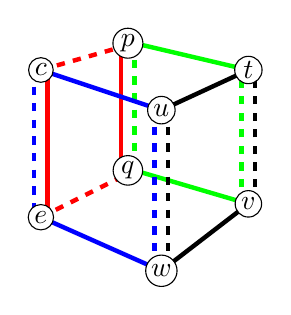
\begin{tikzpicture}[scale=1.7]
\draw[ultra thick, dashed, red] (0,0) -- (0.7,.2);
\draw[ultra thick, red] (0.05,0) -- (0.05,-1.1);
\draw[ultra thick, dashed, blue] (-.05,0) -- (-.05,-1.1);
\draw[ultra thick, dashed, red] (0,-1.1) -- (.7,-.75);
\draw[ultra thick, green] (.7,-.75) -- (1.55,-1);
\draw[ultra thick, dashed, black] (1.6,-1) -- (1.6,0);
\draw[ultra thick, dashed, green] (1.5,-1) -- (1.5,0);
\draw[ultra thick, black] (1.55,0) -- (0.9,-.3);
\draw[ultra thick, blue] (0,-1.1) -- (.9,-1.5);
\draw[ultra thick, black] (.9,-1.5) -- (1.55,-1);
\draw[ultra thick, green] (1.55,0) -- (.7,.2);
\draw[ultra thick, dashed, green] (.7,.2) -- (.7,-.75);
\draw[ultra thick, red] (.6,.2) -- (.6,-.75);
\draw[ultra thick, blue] (0,0) -- (0.9,-.3);
\node[circle, fill=white, draw=black, text=black,  inner sep=1pt] at (0.65,-.75) {$q$};
\draw[ultra thick, dashed, blue] (.85,-.3) -- (.85,-1.5);
\draw[ultra thick, dashed, black] (.95,-.3) -- (.95,-1.5);
\node[circle, fill=white, draw=black, text=black, inner sep=1pt] at (0,0) {$c$}; 
\node[circle, fill=white, draw=black, text=black,  inner sep=1pt] at (0.65,.2) {$p$}; 
\node[circle, fill=white, draw=black, text=black,  inner sep=1pt] at (1.55,0) {$t$};
\node[circle, fill=white, draw=black, text=black, inner sep=1pt] at (.9,-.3) {$u$}; 
\node[circle, fill=white, draw=black, text=black,  inner sep=1pt] at (0,-1.1) {$e$}; 
\node[circle, fill=white, draw=black, text=black, inner sep=1pt] at (1.55,-1) {$v$}; 
\node[circle, fill=white, draw=black, text=black,  inner sep=1pt] at (0.9,-1.5) {$w$}; 
\end{tikzpicture}
